\documentclass{oblivoir}
\usepackage{amsmath,amssymb,amsthm,kotex,mdframed,paralist,chngcntr}
\usepackage{kswrapfig}

\newcounter{num}
%\newcommand{\defi}[1]
%{\bigskip\noindent\refstepcounter{num}\textbf{정의 \arabic{num}) #1}\par}
%\newcommand{\theo}[1]
%{\bigskip\noindent\refstepcounter{num}\textbf{정리 \arabic{num}) #1}\par}
%\newcommand{\exam}[1]
%{\bigskip\noindent\refstepcounter{num}\textbf{예시 \arabic{num}) #1}\par}
\newcommand{\prob}[1]
{\bigskip\noindent\refstepcounter{num}\textbf{문제 \arabic{num}) #1}\par}
%\newcommand{\howo}[1]
%{\bigskip\noindent\refstepcounter{num}\textbf{숙제 \arabic{num}) #1}\par\bigskip}

\newcommand{\ans}{{\raggedleft\textbf{답 : (\qquad\qquad\qquad\qquad\qquad\qquad)}
\par}}

\renewcommand{\proofname}{증명)}
\counterwithout{subsection}{section}


%%%
\begin{document}
\Large

\title{승재 05 - 최고수준 수학}
\author{}
\date{\today}
\maketitle
%\tableofcontents


%
\prob{p103, \#06-1}
\kswrapfig[Pos=r]{103-06-1}{
오른쪽 그림과 같이 한 변의 길이가 \(7\)m인 정사각형 모양인 염소 우리의 한 꼭짓점에 염소 한 마리가 14m의 끈으로 매여 있습니다.
이 염소가 풀을 뜯기 위해 움직일 수 있는 범위의 넓이는 몇 m\(^2\)입니까?
(단, 우리 안으로는 들어갈 수 없고 염소의 길이는 생각하지 않습니다.
원주율 : \(3\frac17\))
}

\ans{}

\newpage

%
\prob{p103, \#06-2}
\kswrapfig[Pos=r]{103-06-2}{
오른쪽 그림과 같이 한 변의 길이가 \(10\)m인 정사각형 모양인 염소 우리의 점에 염소 한 마리가 20m의 끈으로 매여 있습니다.
이 염소가 풀을 뜯기 위해 움직일 수 있는 범위의 넓이는 몇 m\(^2\)입니까?
(단, 우리 안으로는 들어갈 수 없고 염소의 길이는 생각하지 않습니다.
원주율 : \(3\))
}

\ans{}

%
\prob{p103, \#06-3}
\kswrapfig[Pos=r]{103-06-3}{
오른쪽 그림과 같이 한 변의 길이가 \(6\)m인 정삼각형 모양인 염소 우리의 점에 염소 한 마리가 9m의 끈으로 매여 있습니다.
이 염소가 풀을 뜯기 위해 움직일 수 있는 범위의 넓이는 몇 m\(^2\)입니까?
(단, 우리 안으로는 들어갈 수 없고 염소의 길이는 생각하지 않습니다.
원주율 : \(3.1\))
}

\ans{}

%%
%\prob{p103, \#06-4}
%\kswrapfig[Pos=r]{103-06-4}{
%오른쪽 그림과 같이 벽이 염소 한 마리가 \(6\)m인 끈으로 매여 있습니다.
%끈이 매여있는 지점으로부터 8m 떨어진 곳에 먹이가 있을 때, 염소는 먹이에 몇 m까지 가까이 갈 수 있습니까?
%(단, 염소는 벽 안으로는 들어갈 수 없고 염소의 길이는 생각하지 않습니다.
%원주율 : \(3.1\))
%}
%
%\ans{}

\newpage

%
\prob{p126, \#08-1}
\kswrapfig[Pos=r]{126-08-1}{
크기가 같은 정육면체 모양의 쌓기나무 27개를 쌓아서 오른쪽과 같은 큰 정육면체를 만들었더니 겉넓이가 쌓기나무 27개의 겉넓이의 합보다 108cm\(^2\) 줄어들었습니다.
쌓기나무 한 개의 겉넓이는 몇 cm\(^2\) 입니까?
}

\ans{}

%
\prob{p126, \#08-2}
\kswrapfig[Pos=r]{126-08-2}{
크기가 같은 정육면체 모양의 쌓기나무 18개를 쌓아서 오른쪽과 같은 큰 정육면체를 만들었더니 겉넓이가 쌓기나무 18개의 겉넓이의 합보다 16.5cm\(^2\) 줄어들었습니다.
쌓기나무 한 개의 겉넓이는 몇 cm\(^2\) 입니까?
}

\ans{}
\newpage

%
\prob{p126, \#08-3}
\kswrapfig[Pos=r]{126-08-3}{
오른쪽 그림과 같이 정육면체 모양의 쌓기나무 네 개를 이용하여 여러 가지 모양으로 쌓았습니다.
이 중 겉넓이가 다른 하나는 무엇입니까?
}

\ans{}

%
\prob{p126, \#08-4}
아래 그림과 같이 정육면체 모양의 쌓기나무들을 이용하여 (가)와 (나)를 만들었습니다.
(가)의 겉넓이가 (나)의 겉넓이보다 32cm\(^2\)만큼 넓을 때
쌓기나무의 모서리의 길이는 몇 cm입니까?

\begin{figure}[h]
\centering
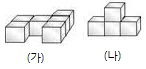
\includegraphics[width=0.5\textwidth]{126-08-4}
\end{figure}

\ans{}

\newpage

%
\prob{p59, \#12-4}
어떤 물건을 원가의 0.4만큼 이익을 붙여 정가를 매겼습니다.
이 물건을 정가의 0.2을 할인하여 팔면 1200원의 이익이 생긴다고 합니다.
이 물건의 원가는 얼마입니까?

\ans{}


%
\prob{p59, \#12-5}
어떤 물건을 원가의 0.4만큼 이익을 붙여 정가를 매겼지만 정가의 0.25을 할인하여 팔기로 했습니다.
이 물건을 250개 팔았을 때 15000원의 이익이 생겼다고 합니다.
이 물건의 원가는 얼마입니까?

\ans{}

%
\prob{p82, \#02-5}
반지름이 \(10\)cm인 원이 있을 때 그 원의 반지름을 한 변으로 하는 정사각형을 만들었습니다.\\
(1) 원래 원의 넓이에 대한 새로 만든 정사각형의 넓이의 비율을 백분율로 나타내시오.\\
(2) 원래 원의 둘레에 대한 새로 만든 정사각형의 둘레의 비율을 백분율로 나타내시오.
(소수 첫째자리에서 반올림합니다. 원주율:3.14)

{\raggedleft\textbf{답 : (1) (\qquad\qquad\qquad)\quad\quad(2) (\qquad\qquad\qquad)}
\par}

%
\prob{p82, \#02-6}
반지름이 10cm인 원의 반지름을 20\%만큼 늘려서 새로운 원을 만들었을 때\\
(1) 원의 넓이는 몇 \%만큼 증가했습니까?\\
(2) 원의 둘레는 몇 \%만큼 증가했습니까?
(원주율:3.14)

{\raggedleft\textbf{답 : (1) (\qquad\qquad\qquad)\quad\quad(2) (\qquad\qquad\qquad)}
\par}

%%
%\prob{p82, \#02-7}
%어떤 정육면체의 한 변의 길이를 20\% 늘려서 새로운 정육면체를 만들었을 때 겉넓이가 88cm\(^2\)만큼 증가했을 때, 원래 정육면체의 한 변의 길이는 몇 cm입니까?

\newpage

%
\prob{p101, \#11-3}
아래 도형은 삼각형 ㄱㄴㄷ를 점 ㄴ을 중심으로 \(45^\circ\)만큼 회전시켜 삼각형 ㄹㄴㅁ를 얻은 것입니다.
색칠한 부분의 넓이는 몇 cm\(^2\)입니까?
(원주율 : 3.14)
\begin{figure}[h]
\centering
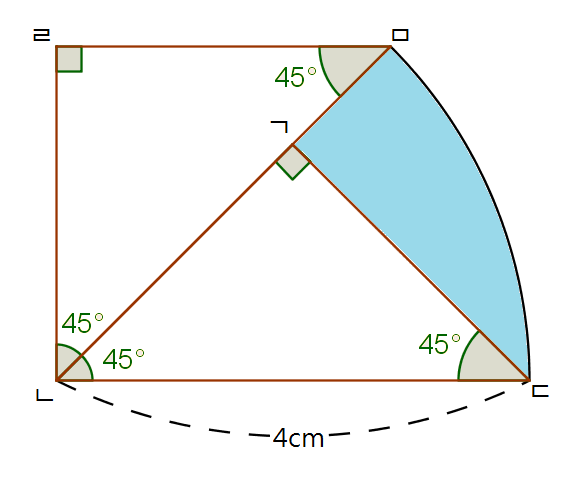
\includegraphics[width=0.5\textwidth]{10111-3}
\end{figure}

\ans{}

\end{document}